\chapter{指针}

\section{指针}

\subsection{指针(Pointer)}

每个变量都会在内存中占用一定的空间,不同类型的变量占用的空间大小也不同。每个空间都有一个地址,一般采用十六进制表示,如0x0060FEFC。\\

有时候需要通过变量的地址对变量进行操作,这时候就需要将变量的地址保存起来,保存地址的变量就成为指针。

\begin{figure}[H]
    \centering
    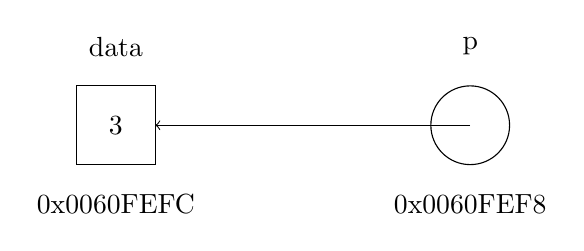
\begin{tikzpicture}
        \draw (0,0) rectangle node{3} (1,1);
        \draw (0.5,1.5) node{data};
        \draw (0.5,-0.5) node{0x0060FEFC};

        \draw (5,0.5) circle (0.5);
        \draw (5,1.5) node{p};
        \draw (5,-0.5) node{0x0060FEF8};

        \draw[->] (5,0.5) -- (1,0.5);
    \end{tikzpicture}
\end{figure}

*用于声明一个指针变量,例如int *p表示p是一个指针,指向一个int类型的变量的地址。通过取地址运算符\&可以获取变量的地址,占位符\%p能够以十六进制的形式输出地址。\\

既然指针保存了另一个变量的地址,那么通过指针就可以访问到那个变量上的数据。在指针变量前使用*运算符,就可以获取到指针所指向的变量的值。

\begin{figure}[H]
    \centering
    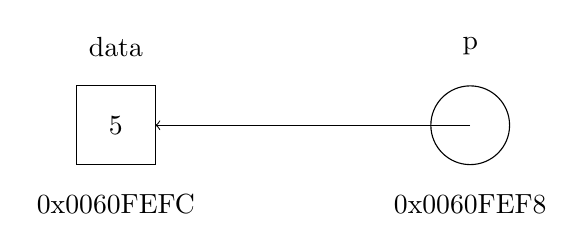
\begin{tikzpicture}
        \draw (0,0) rectangle node{5} (1,1);
        \draw (0.5,1.5) node{data};
        \draw (0.5,-0.5) node{0x0060FEFC};

        \draw (5,0.5) circle (0.5);
        \draw (5,1.5) node{p};
        \draw (5,-0.5) node{0x0060FEF8};

        \draw[->] (5,0.5) -- (1,0.5);
    \end{tikzpicture}
\end{figure}

\mybox{指针}

\begin{lstlisting}[language=C++]
#include <iostream>

using namespace std;

int main() {
    int data = 3;
    int *p = &data;

    cout << "Value of data: " << data << endl;
    cout << "Address of data: " << &data << endl;

    cout << "Value of p: " << p << endl;
    cout << "Address of p: " << &p << endl;
    cout << "Value of data pointed by p: " << *p << endl;
    
    *p = 5;

    cout << "Value of data: " << data << endl;
    cout << "Value of data pointed by p: " << *p << endl;

    return 0;
}
\end{lstlisting}

\begin{tcolorbox}
    \mybox{运行结果}
    \begin{verbatim}
Value of data: 3
Address of data: 0x61fe1c
Value of p: 0x61fe1c
Address of p: 0x61fe10
Value of data pointed by p: 3
Value of data: 5
Value of data pointed by p: 5
	\end{verbatim}
\end{tcolorbox}

为什么不直接修改变量的值,还要多此一举通过指针修改呢?\\

例如需要实现swap()用于交换两个变量的值,由于传递参数是按值传递(pass by value),所以交换的仅仅只是swap()中局部变量的值。\\

这种情况下就需要使用指针,将需要交换的变量的地址传递给swap(),然后在swap()中交换这两个地址上的值。\\

\mybox{交换}

\begin{lstlisting}[language=C++]
#include <iostream>

using namespace std;

void swap(int *data1, int *data2) {
    int temp = *data1;
    *data1 = *data2;
    *data2 = temp;
}

int main() {
    int a = 3;
    int b = 5;

    cout << "Before: a = " << a << ", b = " << b << endl;
    swap(&a, &b);
    cout << "After: a = " << a << ", b = " << b << endl;
    return 0;
}
\end{lstlisting}

\begin{tcolorbox}
    \mybox{运行结果}
    \begin{verbatim}
Before: a = 3, b = 5
After: a = 5, b = 3
	\end{verbatim}
\end{tcolorbox}

函数最多只能返回一个值,但如果需要有多个值需要返回,就可以使用指针将数据带回。\\

\mybox{一元二次方程}

\begin{lstlisting}[language=C++]
#include <iostream>
#include <cmath>
#include <iomanip>

using namespace std;

/**
 * Solve quadratic equation ax^2 + bx + c = 0.
 * @param a coefficient of x^2
 * @param b coefficient of x
 * @param c constant
 * @param x1 pointer to the first root
 * @param x2 pointer to the second root
 * @return true if the equation has real roots, false otherwise.
 */
bool solver(double a, double b, double c, double *x1, double *x2) {
    double delta = b * b - 4 * a * c;
    if (delta < 0) {
        return false;
    }
    *x1 = (-b + sqrt(delta)) / (2 * a);
    *x2 = (-b - sqrt(delta)) / (2 * a);
    return true;
}

int main() {
    double a, b, c;
    double x1, x2;

    cout << "Quadratic equation ax^2 + bx + c = 0" << endl;
    cout << "Enter coefficients a, b, c: ";
    cin >> a >> b >> c;

    if (solver(a, b, c, &x1, &x2)) {
        cout << fixed << setprecision(2) 
             << "x1 = "  << x1 << ", x2 = " << x2 << endl;
    } else {
        cout << "No real roots" << endl;
    }

    return 0;
}
\end{lstlisting}

\begin{tcolorbox}
    \mybox{运行结果}
    \begin{verbatim}
Quadratic equation ax^2 + bx + c = 0
Enter coefficients a, b, c: 1 -9 20
x1 = 5.00, x2 = 4.00
	\end{verbatim}
\end{tcolorbox}

\vspace{0.5cm}

\subsection{NULL}

如果一个变量声明时没有初始化,那么它的值是不确定的。声明指针时如果不对指针进行初始化,那么它就会指向一块不确定的内存地址,这种指针被称为野指针。\\

使用野指针可能会导致程序崩溃,因为它可能指向一个不可访问的内存地址。因此,如果指针没有指向一个确定的内存地址时,应该将其赋值为空指针NULL。

\vspace{-0.5cm}

\begin{lstlisting}[language=C++]
int *p = NULL;
\end{lstlisting}

\newpage

\section{指针与数组}

\subsection{指针与数组}

数组名本质上就是一个指针,它指向数组的首地址。因此在获取数组的地址时,可以不使用\&运算符。\\

\begin{figure}[H]
    \centering
    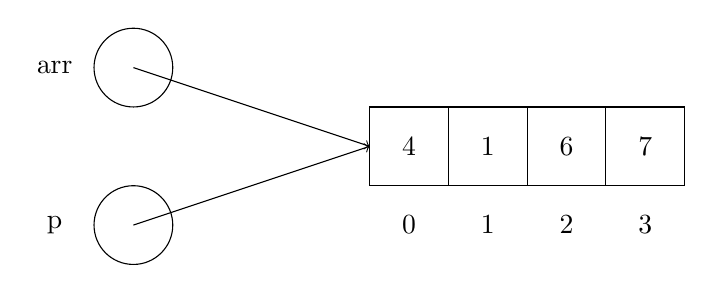
\begin{tikzpicture}
        \draw (0,1) circle (0.5);
        \draw (-1,1) node{arr};

        \draw (0,-1) circle (0.5);
        \draw (-1,-1) node{p};

        \draw (3,-0.5) rectangle (7,0.5);
        \draw (4,-0.5) -- (4,0.5);
        \draw (5,-0.5) -- (5,0.5);
        \draw (6,-0.5) -- (6,0.5);

        \draw (3.5,0) node {4};
        \draw (4.5,0) node {1};
        \draw (5.5,0) node {6};
        \draw (6.5,0) node {7};

        \draw (3.5,-1) node {0};
        \draw (4.5,-1) node {1};
        \draw (5.5,-1) node {2};
        \draw (6.5,-1) node {3};

        \draw[->] (0,1) -- (3,0);
        \draw[->] (0,-1) -- (3,0);
    \end{tikzpicture}
\end{figure}

当对一个指向数组的指针进行加减运算时(如p++和p--),并不是将地址加1或减1,而是根据指针的类型加或减对应字节的长度。例如p是一个int型指针,那么p++会将地址加4(int占4个字节)、p -= 2会将地址减8。\\

\mybox{指针与数组}

\begin{lstlisting}[language=C++]
#include <iostream>

using namespace std;

int main() {
    int arr[] = {4, 1, 6, 7};
    int n = sizeof(arr) / sizeof(arr[0]);
    int *p = arr;

    cout << "Address of arr: " << arr << endl;
    for (int i = 0; i < n; i++) {
        cout << "Address of arr[" << i << "]: " << &arr[i] << endl;
    }

    cout << "Value of p: " << p << endl;
    for (int i = 1; i < n; i++) {
        cout << "Value of p + " << i << ": " << p + i << endl;
    }

    *p = 9;
    *(p + 1) = 8;
    *(p + 2) = 7;
    *(p + 3) = 6;

    for (int i = 0; i < n; i++) {
        cout << "arr[" << i << "]: " << arr[i] << endl;
    }

    return 0;
}
\end{lstlisting}

\begin{tcolorbox}
    \mybox{运行结果}
    \begin{verbatim}
Address of arr: 0x61fdf0   
Address of arr[0]: 0x61fdf0
Address of arr[1]: 0x61fdf4
Address of arr[2]: 0x61fdf8
Address of arr[3]: 0x61fdfc
Value of p: 0x61fdf0
Value of p + 1: 0x61fdf4
Value of p + 2: 0x61fdf8
Value of p + 3: 0x61fdfc
arr[0]: 9
arr[1]: 8
arr[2]: 7
arr[3]: 6
	\end{verbatim}
\end{tcolorbox}

\vspace{0.5cm}

\subsection{数组与函数}

数组作为函数参数时,会将数组的地址传递给函数,函数接收到的是一个指向数组首地址的指针。由于在函数中失去了数组长度的信息,并不能通过sizeof()计算出数组的长度(计算得到的是一个指针变量所占的空间),因此将数组传入函数时,还需要将其长度一并作为参数传给函数。\\

\mybox{查找}

\begin{lstlisting}[language=C++]
#include <iostream>

using namespace std;

int search(int *arr, int n, int key) {
    for (int i = 0; i < n; i++) {
        if (arr[i] == key) {
            return i;
        }
    }
    return -1;
}

int main() {
    int arr[] = {4, 7, 1, 3, 9, 2};
    int n = sizeof(arr) / sizeof(arr[0]);

    int index = search(arr, n, 3);
    if (index == -1) {
        cout << "Not found" << endl;
    } else {
        cout << "Found at index " << index << endl;
    }

    return 0;
}
\end{lstlisting}

\begin{tcolorbox}
    \mybox{运行结果}
    \begin{verbatim}
Found at index 3
	\end{verbatim}
\end{tcolorbox}

\newpage

\section{指针与字符串}

\subsection{指针与字符串}

数组和指针都可以用于定义一个字符串,但是它们内存分配的方式不同,从而导致它们的使用方式也不同。\\

以数组形式定义的字符串,每个字符保存在一个字符数组中。这样的字符串是可以修改的,与普通的数组类似。\\

但是如果让一个指针指向一个字符串,那么这个字符串会被存储在常量区。常量区中的数据是不可以修改的,因此使用指针去修改字符串会导致程序崩溃。\\

\begin{figure}[H]
    \centering
    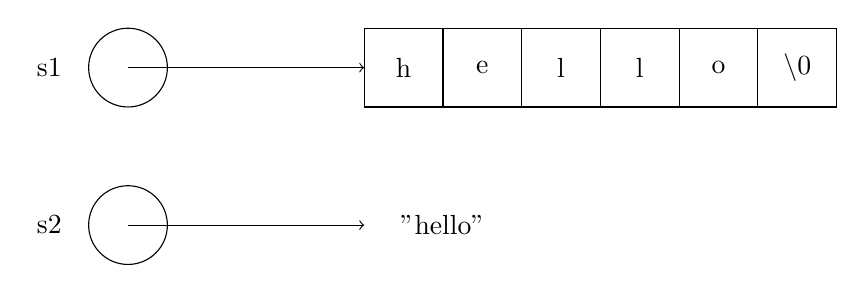
\begin{tikzpicture}
        \draw (0,0) circle (0.5);
        \draw (-1,0) node{s1};

        \draw (3,-0.5) rectangle (9,0.5);
        \draw (4,-0.5) -- (4,0.5);
        \draw (5,-0.5) -- (5,0.5);
        \draw (6,-0.5) -- (6,0.5);
        \draw (7,-0.5) -- (7,0.5);
        \draw (8,-0.5) -- (8,0.5);

        \draw (3.5,0) node {h};
        \draw (4.5,0) node {e};
        \draw (5.5,0) node {l};
        \draw (6.5,0) node {l};
        \draw (7.5,0) node {o};
        \draw (8.5,0) node {$ \backslash $0};

        \draw[->] (0,0) -- (3,0);

        \draw (0,-2) circle (0.5);
        \draw (-1,-2) node{s2};
        \draw (4,-2) node {"hello"};
        \draw[->] (0,-2) -- (3,-2);
    \end{tikzpicture}
\end{figure}

\vspace{-0.5cm}

\begin{lstlisting}[language=C++]
char s1[] = "hello";
s1[0] = 'H';
cout << s1 << endl;

char *s2 = "hello";
s2[0] = 'H';        // error
cout << s2 << endl;
\end{lstlisting}

在对指向字符串的指针进行赋值操作的时候,并不会产生新的字符串,只是让两个指针都指向同一个字符串,对任意一个指针做的操作都会影响另一个指针。\\

\begin{figure}[H]
    \centering
    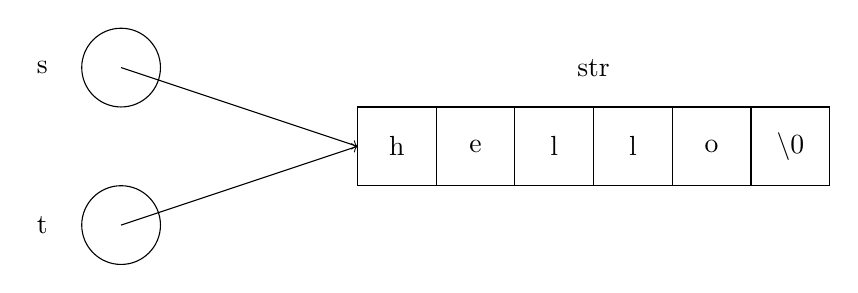
\begin{tikzpicture}
        \draw (0,1) circle (0.5);
        \draw (-1,1) node{s};

        \draw (0,-1) circle (0.5);
        \draw (-1,-1) node{t};

        \draw (3,-0.5) rectangle (9,0.5);
        \draw (4,-0.5) -- (4,0.5);
        \draw (5,-0.5) -- (5,0.5);
        \draw (6,-0.5) -- (6,0.5);
        \draw (7,-0.5) -- (7,0.5);
        \draw (8,-0.5) -- (8,0.5);

        \draw (3.5,0) node {h};
        \draw (4.5,0) node {e};
        \draw (5.5,0) node {l};
        \draw (6.5,0) node {l};
        \draw (7.5,0) node {o};
        \draw (8.5,0) node {$ \backslash $0};
        \draw (6,1) node {str};

        \draw[->] (0,1) -- (3,0);
        \draw[->] (0,-1) -- (3,0);
    \end{tikzpicture}
\end{figure}

\mybox{指向字符串的指针}

\begin{lstlisting}[language=C++]
#include <iostream>

using namespace std;

int main() {
    char str[] = "hello";
    char *s = str;
    char *t = s;

    s[0] = 'H';
    cout << "s = " << s << endl;
    cout << "t = " << t << endl;

    return 0;
}
\end{lstlisting}

\begin{tcolorbox}
    \mybox{运行结果}
    \begin{verbatim}
s = Hello
t = Hello
	\end{verbatim}
\end{tcolorbox}

\newpage

\section{二级指针}

\subsection{二级指针(Pointer to pointer)}

既然指针也是一个变量,那么一个指针也可以指向另一个指针,这样的指针称为二级指针。

\begin{figure}[H]
    \centering
    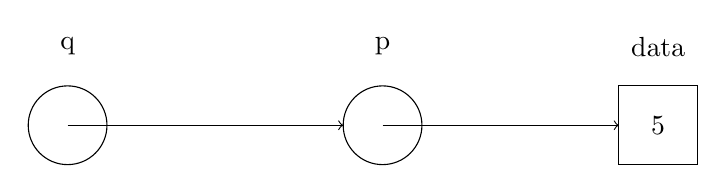
\begin{tikzpicture}
        \draw (0,0) circle (0.5);
        \draw (0,1) node{q};
        \draw (4,0) circle (0.5);
        \draw (4,1) node{p};

        \draw (7,-0.5) rectangle (8,0.5);
        \draw (7.5,0) node {5};
        \draw (7.5,1) node {data};

        \draw[->] (0,0) -- (3.5,0);
        \draw[->] (4,0) -- (7,0);
    \end{tikzpicture}
\end{figure}

其中p是一个int型的指针(int *),指向了data;q是一个指向int型指针的指针(int **),即q指向了一个指向int的指针。\\

\mybox{二级指针}

\begin{lstlisting}[language=C++]
#include <iostream>

using namespace std;

int main() {
    int data = 5;
    int *p = &data;
    int **q = &p;

    cout << "data = " << data << endl;
    cout << "*p = " << *p << endl;
    cout << "**q = " << **q << endl;

    cout << "Address of data = " << &data << endl;
    cout << "Address of p = " << &p << endl;
    cout << "Address of q = " << &q << endl;

    cout << "Value of p = " << p << endl;
    cout << "Value of q = " << q << endl;

    return 0;
}
\end{lstlisting}

\begin{tcolorbox}
    \mybox{运行结果}
    \begin{verbatim}
data = 5
*p = 5  
**q = 5
Address of data = 0x61fe1c
Address of p = 0x61fe10
Address of q = 0x61fe08
Value of p = 0x61fe1c
Value of q = 0x61fe10
	\end{verbatim}
\end{tcolorbox}

\vspace{0.5cm}

\subsection{指针与二维数组}

二级指针还可以用于表示二维数组。与一维数组类似,可以使用下标或*运算符来访问二维数组中的元素。\\

\begin{figure}[H]
    \centering
    \begin{tikzpicture}
        \draw (0,1.5) circle (0.5);
        \draw (0,2.5) node{arr};
        \draw (4,1.5) circle (0.5);

        \draw (7,-2) rectangle (11,2);
        \draw (8,-2) -- (8,2);
        \draw (9,-2) -- (9,2);
        \draw (10,-2) -- (10,2);
        \draw (7,-1) -- (11,-1);
        \draw (7,0) -- (11,0);
        \draw (7,1) -- (11,1);

        \draw[->] (0,1.5) -- (3.5,1.5);
        \draw[->] (4,1.5) -- (7,1.5);
    \end{tikzpicture}
\end{figure}

例如,arr[2][1]也可以写成*(*(arr + 2) + 1)。

\begin{figure}[H]
    \centering
    \begin{tikzpicture}
        \draw (0,1.5) circle (0.5);
        \draw (0,2.5) node{arr};
        \draw (4,1.5) circle (0.5);

        \draw (7,-2) rectangle (11,2);
        \draw (8,-2) -- (8,2);
        \draw (9,-2) -- (9,2);
        \draw (10,-2) -- (10,2);
        \draw (7,-1) -- (11,-1);
        \draw (7,0) -- (11,0);
        \draw (7,1) -- (11,1);

        \draw[->] (0,1.5) -- (3.5,1.5);
        \draw[->] (4,1.5) -- (8.5,-0.5);
    \end{tikzpicture}
\end{figure}

当如果命令行运行时,可以向main()函数传递命令行参数。传递参数的数量和值可以通过argc(argument count)和argv(argument vector)来获取。argv为一个二维数组,每个元素都是一个字符串,其中argv[0]为当前程序的名称。\\

\mybox{命令行参数}

\begin{lstlisting}[language=C++]
#include <iostream>
#include <cctype>
#include <cstring>

using namespace std;

char *lower(char *s) {
    char *p = s;
    while (*p) {
        *p = tolower(*p);
        p++;
    }
    return s;
}

char *upper(char *s) {
    char *p = s;
    while (*p) {
        *p = toupper(*p);
        p++;
    }
    return s;
}

void usage(const char *program) {
    cout << "Usage: " << program << " [option] [string]" << endl;
    cout << "--lower: convert string to lower case" << endl;
    cout << "--upper: convert string to upper case" << endl;
}

int main(int argc, char **argv) {
    if (argc != 3) {
        usage(argv[0]);
        return 1;
    }

    char *option = argv[1];
    char *string = argv[2];

    if (strcmp(option, "--lower") == 0) {
        cout << "Lower: " << lower(string) << endl;
    } else if (strcmp(option, "--upper") == 0) {
        cout << "Upper: " << upper(string) << endl;
    } else {
        usage(argv[0]);
        return 1;
    }

    return 0;
}
\end{lstlisting}

\begin{lstlisting}
g++ -Wall command_line.cpp -o command_line
./command_line --upper "Hello World!"
\end{lstlisting}

\begin{tcolorbox}
    \mybox{运行结果}
    \begin{verbatim}
Upper: HELLO WORLD!
	\end{verbatim}
\end{tcolorbox}

\newpage

\section{动态内存申请}

\subsection{内存管理}

计算机的内存主要包括:

\begin{enumerate}
    \item 代码区:存储程序执行时使用的指令。
    \item 数据区:存储程序运行时使用的全局变量和静态变量。
    \item 栈区(stack):存储函数调用时使用的局部变量,栈中的内存由编译器自动分配和释放。
    \item 堆区(heap):存储动态分配内存的变量,需要由程序员自己分配和释放。
\end{enumerate}

\begin{figure}[H]
    \centering
    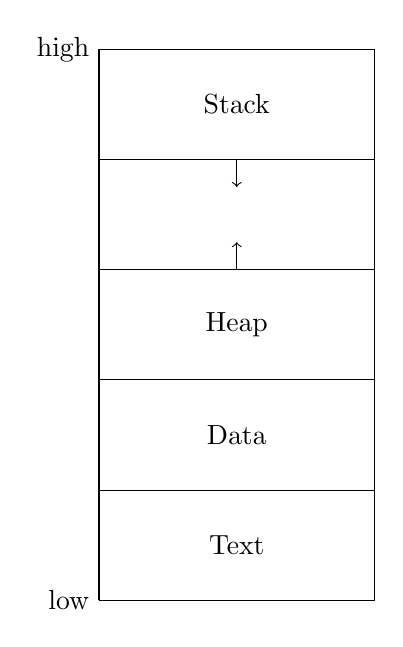
\begin{tikzpicture}[scale=0.7]
        \draw[-] (0,0) -- (0,10) -- (5,10) -- (5,0) -- (0,0);
        \draw[-] (0,2) -- (5,2);
        \draw[-] (0,4) -- (5,4);
        \draw[-] (0,6) -- (5,6);
        \draw[-] (0,8) -- (5,8);

        \draw (0,0) node[left] {low};
        \draw (0,10) node[left] {high};

        \draw (2.5,1) node {Text};
        \draw (2.5,3) node {Data};
        \draw (2.5,5) node {Heap};
        \draw (2.5,9) node {Stack};

        \draw[->] (2.5,8) -- (2.5,7.5);
        \draw[->] (2.5,6) -- (2.5,6.5);
    \end{tikzpicture}
    \caption{内存区域}
\end{figure}

有时候需要在函数中生成一个数组,并且将数组返回给调用者。但是在函数内定义的数组是局部变量,存储于栈区。函数执行完毕后,数组所占用的内存空间会被释放。因此被返回的数组的指针指向的是一个已经被释放的内存空间,这样就会导致程序崩溃。\\

另一种情况是,由于数组一旦声明后,其容量就不能再改变。当需要在运行时动态改变数组容量时,就可以采用动态内存申请的方式。\\

\subsection{malloc()}

malloc()函数定义在<cstdlib>中,用于在堆区申请一块内存空间,其函数原型为:

\vspace{-0.5cm}

\begin{lstlisting}[language=C++]
void* malloc(size_t size);
\end{lstlisting}

malloc()接受一个参数size,表示申请空间的大小(单位:字节),并返回指向申请到的空间的首地址的指针。如果申请失败,则返回NULL。\\

malloc()返回的是无类型指针void *,这是由于malloc()只负责申请指定大小的空间,并不关心这块空间将会被存放什么类型的数据。因此,开发者需要自行将其转换为对应的类型。\\

\mybox{内存}

\begin{lstlisting}[language=C++]
#include <iostream>
#include <cstdlib>

using namespace std;

int main() {
    void *p;
    int cnt = 0;

    // allocate 100MB memory each time
    while ((p = malloc(100 * 1024 * 1024))) {
        cnt++;
    }
    cout << "Allocated " << cnt * 100 << " MB memory" << endl;

    return 0;
}
\end{lstlisting}

\begin{tcolorbox}
    \mybox{运行结果}
    \begin{verbatim}
Allocated 57700 MB memory
	\end{verbatim}
\end{tcolorbox}

\vspace{0.5cm}

\subsection{free()}

通过动态申请来的内存空间需要是需要归还给操作系统,因此需要程序员自行在不需要使用时将其释放。如果不释放内存,这些动态申请的内存空间就会一直占用着,直到程序结束统一被操作系统释放。\\

不释放内存会导致内存泄漏(memory leak),如果一直分配内存而不是释放,最终将会耗尽所有可用的内存,导致程序运行变慢或者崩溃。\\

free()函数用于释放动态申请的内存空间,其接受一个参数ptr,表示要释放的内存空间的首地址。其函数原型为:

\vspace{-0.5cm}

\begin{lstlisting}[language=C++]
void free(void *ptr);
\end{lstlisting}

\vspace{0.5cm}

\mybox{斐波那契数列}

\begin{lstlisting}[language=C++]
#include <iostream>
#include <cstdlib>

using namespace std;

int *generate_fibonacci(int n) {
    int *arr = (int *)malloc(n * sizeof(int));
    if (!arr) {
        return NULL;
    }

    arr[0] = 1;
    arr[1] = 1;
    for (int i = 2; i < n; i++) {
        arr[i] = arr[i - 1] + arr[i - 2];
    }
    return arr;
}

int main() {
    int n = 10;
    int *arr = generate_fibonacci(n);

    for (int i = 0; i < n; i++) {
        cout << arr[i] << " ";
    }
    cout << endl;

    free(arr);
    return 0;
}
\end{lstlisting}

\begin{tcolorbox}
    \mybox{运行结果}
    \begin{verbatim}
1 1 2 3 5 8 13 21 34 55
	\end{verbatim}
\end{tcolorbox}

\vspace{0.5cm}

\subsection{calloc()}

calloc()与malloc()功能类似,也是用于动态申请内存空间的。只是malloc()只接受一个参数作为申请空间的大小,申请到的空间并不会进行初始化;而calloc()接受两个参数,可以申请多个指定大小的空间,并将这些空间初始化为0。calloc()的函数原型为:

\vspace{-0.5cm}

\begin{lstlisting}[language=C++]
void *calloc(size_t nitems, size_t size);
\end{lstlisting}

例如需要申请一个长度为n的int数组,并将其初始化为0:

\vspace{-0.5cm}

\begin{lstlisting}[language=C++]
int *arr = (int *)calloc(n, sizeof(int));
\end{lstlisting}

\vspace{0.5cm}

\subsection{realloc()}

realloc()用于对已经动态申请的内存空间进行重新分配(扩容/缩小),其函数原型为:

\vspace{-0.5cm}

\begin{lstlisting}[language=C++]
void *realloc(void *ptr, size_t size);
\end{lstlisting}

realloc()接受两个参数,第一个参数ptr指向需要重新分配内存空间,第二个参数size表示重新分配空间的大小(单位:字节)。realloc()会将原来内存块中的数据复制到新分配的内存块中,并返回指向新内存块的指针。如果重新分配失败,则返回NULL。\\

\mybox{strip}

\begin{lstlisting}[language=C++]
#include <iostream>
#include <cstdlib>
#include <cstring>
#include <cctype>

using namespace std;

char *strip(char *str) {
    int i = 0;
    int j = strlen(str) - 1;

    while (isspace(str[i]) && str[i] != '\0') {
        i++;
    }

    while (isspace(str[j]) && j >= 0) {
        j--;
    }

    int k = 0;
    while (i <= j) {
        str[k++] = str[i++];
    }
    str[k] = '\0';

    str = (char *)realloc(str, (k + 1) * sizeof(char));
    return str;
}

int main() {
    int len = 32;
    char *str = (char *)calloc(len + 1, sizeof(char));

    strcpy(str, "     Hello World! \n\t ");
    cout << "Before: [" << str << "]" << endl;

    str = strip(str);

    cout << "After: [" << str << "]" << endl;

    free(str);
    return 0;
}
\end{lstlisting}

\begin{tcolorbox}
    \mybox{运行结果}
    \begin{verbatim}
Before: [     Hello World! 
     ]
After: [Hello World!]
	\end{verbatim}
\end{tcolorbox}

\newpage